\chapter{Test of effect run time}\label{app:effect_run_time}
A test was made to get a view of the time consumption of each effect.

\section*{Materials and setup}
To measure the time consumption of each effect, the following materials are used:
\begin{itemize}
\item Digilent Analog Discovery 2 (Oscilloscope)
\item Digilent Waveforms 2015 (PC - software)
\item Ezdsp board
\end{itemize}


\begin{figure}[htbp!]
	\centering
		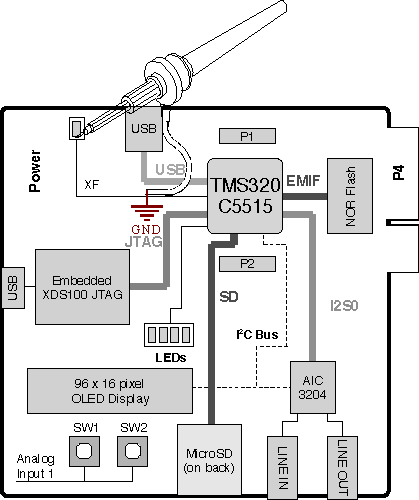
\includegraphics[width=0.5\textwidth]{run_time.pdf}
		\caption{Illustration of the measuer point on the Ezdsp}
		\label{fig:run_time_test_point}
\end{figure}

\includeCode{mainas.asm}{assembly}{12}{21}{Example of run time testing main program}{code:mainas_asm}{code/design/}

\section*{Test procedure}
\begin{enumerate}
\item The materials are set up as in \autoref{fig:run_time_test_point}.
\item The Digilent Waveform 2015 is set as a Scope.
\item  The XF led bit is set at the beginning of the program and cleared in the end of the program, in the mainas file, see example \autoref{code:mainas_asm}.
\item  The Scope is then used to measure the XF LED on time 
\item The data is plotted in MATLAB.
\end{enumerate}

\section*{Reverb run time}
The following measurement \autoref{fig:reverb_time_test} shows the \gls{reverb} program run time.
\begin{figure}[htbp!]
	\centering
		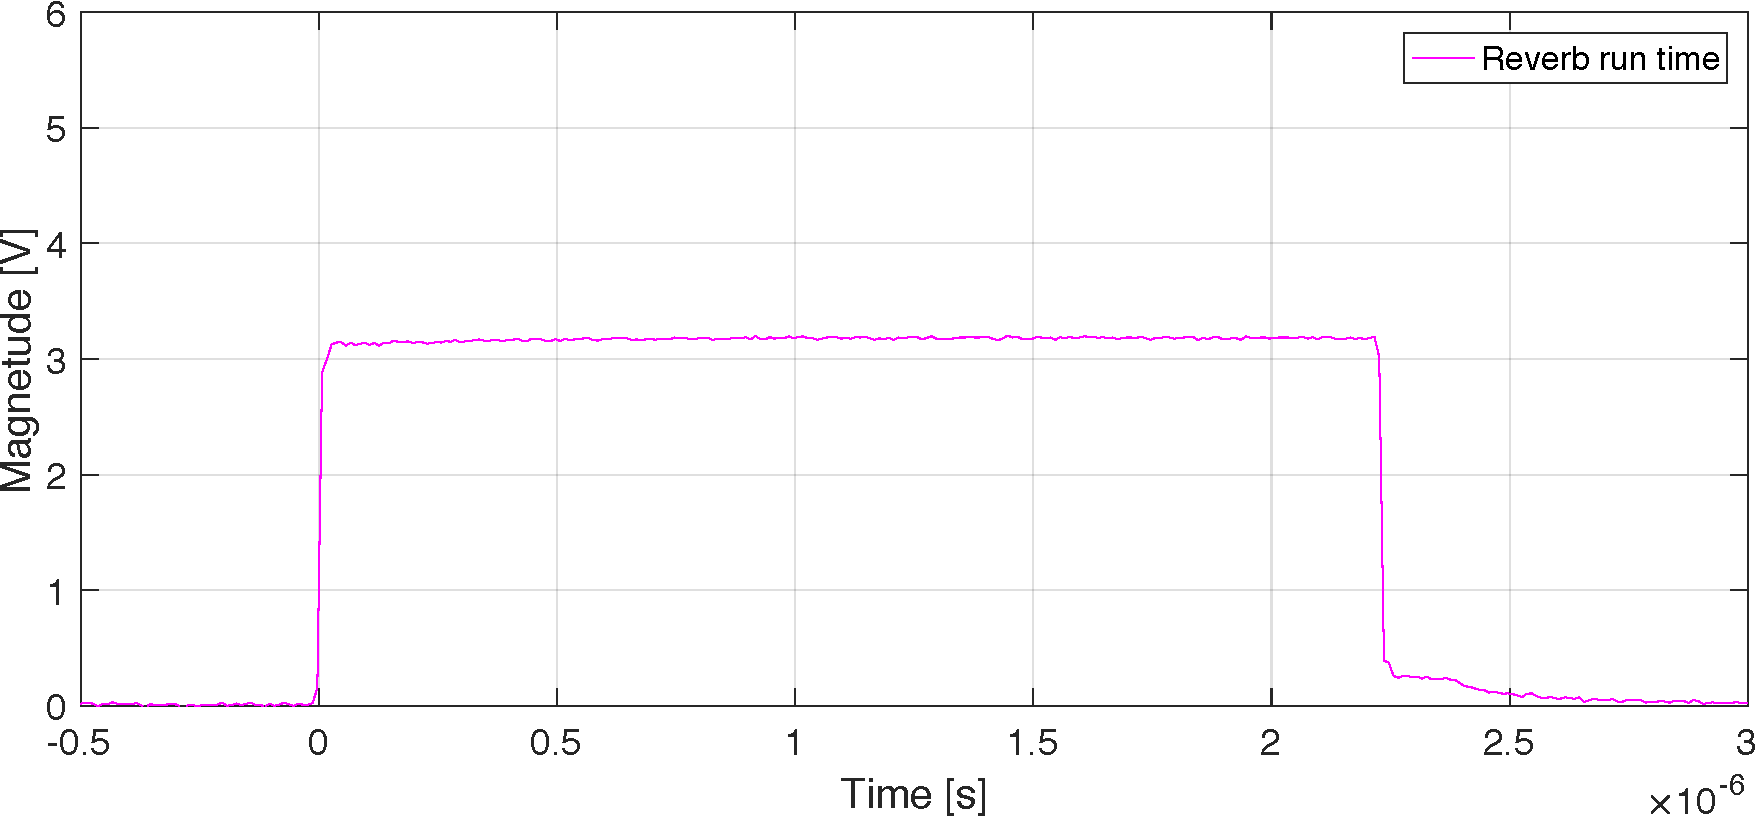
\includegraphics[width=1\textwidth]{reverb_run_time.pdf}
		\caption{The figure shows the run time of the \gls{reverb} assembly program}
		\label{fig:reverb_time_test}
\end{figure}